\normaltrue
\correctiontrue

%\UPSTIidClasse{11} % 11 sup, 12 spé
%\newcommand{\UPSTIidClasse}{12}

\exer{Mouvement TR  $\star$ \label{C2:08:06}}
\setcounter{numques}{0}
\UPSTIcompetence[2]{C2-08}
\UPSTIcompetence[2]{C2-09}
\index{Compétence C2-08}
\index{Compétence C2-09}
\index{Torseur cinétique}
\index{Torseur dynamique}
\index{Mécanisme à 1 translation et 1 rotation}
\ifcorrection
\else
\textbf{Pas de corrigé pour cet exercice.}
\fi

\ifprof
\else
Soit le mécanisme suivant. On a $\vect{AB}=\lambda(t)\vect{i_0}$ et $\vect{BC}=R\vect{i_2}$ avec $R=\SI{30}{mm}$.
De plus :
\begin{itemize}
\item $G_1=B$ désigne le centre d'inertie de \textbf{1}, on note $m_1$ la masse de \textbf{1} et $\inertie{G_1}{1}=\matinertie{A_1}{B_1}{C_1}{0}{0}{0}{\bas{1}}$; 
\item $G_2=C$ désigne le centre d'inertie de \textbf{2}, on note $m_2$ la masse de \textbf{2} et $\inertie{G_2}{2}=\matinertie{A_2}{B_2}{C_2}{0}{0}{0}{\bas{2}}$.
\end{itemize}
\begin{center}
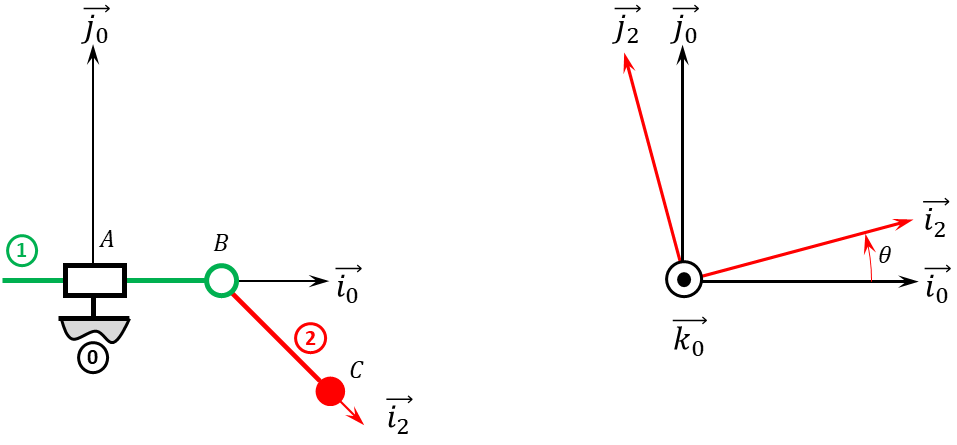
\includegraphics[width=\linewidth]{06_TR_01}
\end{center}
\fi

\question{Exprimer le torseur dynamique $\torseurdyn{2}{0}$ en $B$.}
\ifprof

\textbf{Expression de la résultante dynamique}
$\vectrd{2}{0}=m_2\vectg{G_2}{2}{0} = m_2\dderiv{\vect{AC}}{\rep{0}}$
$\dderiv{\vect{AC}}{\rep{0}}= \dderiv{\vect{AB}}{\rep{0}}+\dderiv{\vect{BC}}{\rep{0}}$
$= \ddot{\lambda}(t) \vect{i_0} + R \dderiv{\vi{2}}{\rep{0}}$
$= \ddot{\lambda}(t) \vect{i_0} + R \deriv{\dot{\theta} \vj{2}}{\rep0}$
$= \ddot{\lambda}(t) \vect{i_0} + R \left(\ddot{\theta} \vj{2} - \dot{\theta}^2 \vi{2}\right) $.



\textbf{Méthode 1 : Calcul en $G_2=C$ puis déplacement du torseur dynamique}
\begin{itemize}
\item Calcul du moment cinétique en $G_2$ : $G_2=C$ est le centre de gravité donc $\vectmc{C}{2}{0}=\inertie{C}{2}\dot{\theta}\vect{k_0} = C_1  \dot{\theta} \vk{1}$.
\item Calcul du moment dynamique en $G_2$ : $G_2=C$ est le centre de gravité donc $\vectmd{C}{2}{0}=\deriv{\vectmc{C}{2}{0}}{\rep{0}}= C_1  \ddot{\theta} \vk{1}$.
\item Calcul du moment dynamique en $B$ : $\babard{B}{C}{2}{0} = C_1  \ddot{\theta} \vk{1} + R\vi{2}\wedge\left(  \ddot{\lambda}(t) \vect{i_0} + R \left(\ddot{\theta} \vj{2} - \dot{\theta}^2 \vi{2}\right)\right)$
$= C_1  \ddot{\theta} \vk{1} + R\left( -\sin \theta \ddot{\lambda}(t) \vk{0} + R \ddot{\theta} \vk{2}\right)$.
\end{itemize}

Au final, on a donc $\torseurdyn{2}{0}=\torseurl{%
m_2\left(\ddot{\lambda}(t) \vect{i_0} + R \left(\ddot{\theta} \vj{2} - \dot{\theta}^2 \vi{2}\right)\right)
}{%
C_1  \ddot{\theta} \vk{1} + R\left( -\sin \theta \ddot{\lambda}(t) \vk{0} + R \ddot{\theta} \vk{2}\right)
}{B}$.
\else
\fi

\question{Déterminer $\vectrd{1+2}{0}\cdot \vect{i_0}$}
\ifprof

On a $\vectrd{1+2}{0}=\vectrd{1}{0}+\vectrd{2}{0}=m_1\ddot{\lambda}(t)\vi{0}+m_2\left(\ddot{\lambda}(t) \vect{i_0} + R \left(\ddot{\theta} \vj{2} - \dot{\theta}^2 \vi{2}\right)\right)$.
On projette alors sur $\vect{i_0}$,
$\vectrd{1+2}{0}\cdot \vect{i_0} =m_1\ddot{\lambda}(t)+m_2\left(\ddot{\lambda}(t)-R \left(\ddot{\theta} \sin\theta(t)  + \dot{\theta}^2 \cos\theta \right)\right) $.
\else
\fi

\ifprof
\else
\footnotesize
\ifcolle
\else
\begin{center}
\begin{tabular}{|p{.9\linewidth}|}
\hline
Indications :
\begin{enumerate}
\item $\torseurdyn{2}{0}=\torseurl{\ddot{\lambda}(t) \vect{i_0} + R \left(\ddot{\theta} \vj{2} - \dot{\theta}^2 \vi{2}\right)}{C_1  \ddot{\theta} \vk{1} + R\left( -\sin \theta \ddot{\lambda}(t) \vk{0} + R \ddot{\theta} \vk{2}\right)}{B}$.
\item $\vectrd{1+2}{0}\cdot \vect{i_0}=m_1\ddot{\lambda}(t)+m_2\left(\ddot{\lambda}(t)- R \left(\ddot{\theta} \sin\theta(t)  + \dot{\theta}^2 \cos\theta \right)\right)$. 
\end{enumerate} \\ \hline
\end{tabular}
\end{center}
\normalsize
\fi
\begin{flushright}
\footnotesize{Corrigé  voir \ref{C2:08:06}.}
\end{flushright}%
\fi